\documentclass[11pt]{article}
\usepackage[utf8]{inputenc}
\usepackage{pgfplots}
\pgfplotsset{width=10cm,compat=1.9}
\usepackage[a4paper, total={6in, 8in}]{geometry}
\usepgfplotslibrary{external}
\tikzexternalize
\title{EE603: Lecture 14 Notes}
\author{Aashish Patel \& Prateek Jain }
\date{October 2021}

\begin{document}

\maketitle

\section{Non-Linear Classification}
\begin{figure}[htp]
    \centering
    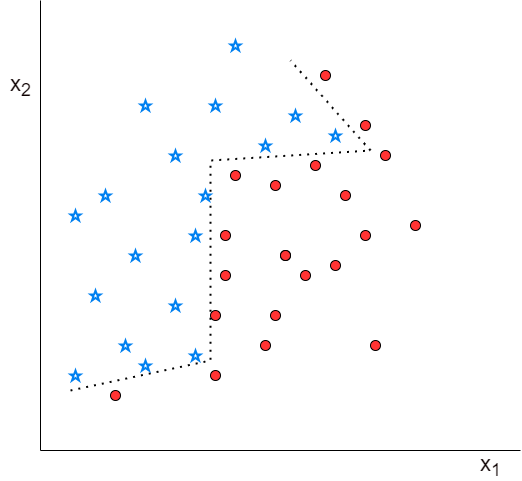
\includegraphics[width=6cm]{fig1.png}
    \caption{A non-linear classifier}
    \label{fig:intro}
\end{figure}
    \subsection{Multiclass Classification}
    \begin{itemize}
        \item {\textbf{Definition:}} Out of multiple given classes, only one class is true. We want our classifier to detect which class is true

\item {\textbf{Input}:} Let us call it vector \textbf{x}

\item {\textbf{Output:}} If there are C classes, the output of the model is \textbf{h}, or $h\sb{c}$, where c= 0,1,2,..., C-1.
Apply softmax on h to get the final output $\textbf{y}$
\begin{center}

$\textbf{y}=softmax(\textbf{h})$\\
\large {\bf {$y\sb{c} = \frac{exp(h\sb{c})}{\sum_{c'}exp(h\sb{c'})}$}} 
\end{center}

\item {\textbf{Target:}} Target is a one-hot vector of size C
\item {\textbf{Example:}} The classification problem where we are given three kinds of flowers and we have to identify the type flower i.e. whether it is Rose or Lotus or Jasmine given height and width as the input
Here C=3 and classes are Rose, Lotus, and Jasmine

\item{\textbf{Some Observations}}
\begin{itemize}
    \item {\bf Why exp in softmax?}
    \begin{itemize}
        \item Derivative of \textit{\bf sigmoid} will be very small so it won't be able to learn properly. Basically if our error function is something that is not very steep i.e. it is very shallow then it won't learn very fast and there are also of noise etc.
        \item But using an exponential function makes it steeper. Any differences are exaggerated by an exponential function( but they are suppressed by the sigmoid function).
        \item 
        Hence, if the derivative is greater than one the differences are exaggerated else if a derivative is less than one the differences are suppressed and sigmoid function derivative is very small therefore the differences are very much suppressed but on the other hand in the exponential function derivative is very large, hence differences are further magnified. That's is why the exponential function very well resembles the \textit{Argmax} function.
    \end{itemize}
\underline{\bf Takeaway}: If we want to exaggerate the differences use an exponential function and if we want to suppress the differences, use a \textit{sigmoid} or \textit{logarithm} as \textit{logarithm} also suppresses the difference.
\end{itemize}

% \begin{tikzpicture}
% \begin{axis}
% \addplot[color=red]{log(x)};
% \end{axis}
% \end{tikzpicture}


\item{\textbf{Loss function}}
\begin{center}
    \large\bf  $\sum_{c}y\sb{c} = 1$ and $\sum_{c}t\sb{c} = 1$
\end{center}
     We need a stronger pull to 0 or 1\\
     Categorical cross-entropy loss function can be used for training.
    \begin{center}
    \large $E\sb{X\sb{ent}} = -\sum_{c}^{} t\sb{c}\cdot log(y\sb{c})$\\
    \end{center}

\item{\textbf{Some Observations}}
\begin{itemize}
    \item{\bf Why not use Mean Squared Error(MSE) as the loss function?}

The derivatives are very small. The mean squared error leads to poor learning since it's a quadratic function and the derivatives are not sufficient to pull our weights to the right value, so we need a stronger pull to zero or one. Also, Mean squared error is good for the continuous approximation such as in regression problems but in the case of multi-class classification answers are discrete i.e. either 0 or 1 ideally. Therefore, we want a very strong pull to these discrete values that's why we don't use the mean squared error function as the loss function.
\\
\item {\bf Why can't we use single output \{0,1,2\} to represent the classes instead of using 3 neurons in the one-hot vector?}
\begin{figure}[htp]
    \centering
    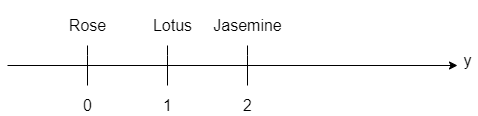
\includegraphics[width=6cm]{fig2.png}
    \caption{A representation of classes}
    \label{fig:line}
\end{figure}

There is an inherent flaw in this representation: 
In the first representation (Figure 2), let us say we have roses, lotuses, and  jasmine. Now, if the output y = \{0,1, 2\} , in other words if the detected class is rose, model will output y=1, if lotus output will be y=2 and for jasmine output y=3.
This implies that rose is much more similar to lotus than to jasmine(since 1 is closer to to 2 than 3) and similarly,  jasmine is much more similar to lotus than rose in this representation.
But one-hot representation does not give any distance preference to any of the classes
\end{itemize}
\end{itemize}

\newpage


%%-------------------------------------------------------------------------
\subsection{Multilabel Classification}
 \begin{itemize}
        \item {\textbf{Definition:}} To detect which attributes(labels) are present in an entity out of some given attributes is known as multilabel classification. 
These labels are independent of each other i.e. any of them can be true or false independent of the other labels.


\item {\textbf{Input}:} Let us call it vector \textbf{x}
\item {\textbf{Output:}} If there are total L labels, the output of the model is \textbf{h} or  $h\sb{l}$ where l= 0,1,2,...,L-1.
Apply sigmoid on h to get the final output $y$
\begin{center}
$\large \textbf{y}=sigmoid(\textbf{h})$\\
\LARGE $y\sb{c}= \frac{1}{1+e^{-h\sb{l}}}$\\
\end{center}
\item {\textbf{Target:}} Target is a multi-hot vector of size L

\item{\textbf{Example}}:  \underline{Face classification}: A face may have different attributes. we want the classifier given a face as the input to detect whether those attributes are present or not 
 
i.e.  we can define different binary attributes
e.g. does a person have a beard, 
does a person wear glasses, 
does a person have hair, 
does a person have moustache, 
does a person have lipstick, 
It can be observed these attributes are independent of each other as a person with a beard can wear glasses or not wear glasses with equal probability

\item{\textbf{Loss function}}
Probabilistic interpretation: 
\begin{center}
$P(l=1) = y\sb{l}$ \\
$P(l=0) = 1-y\sb{l}$
\end{center}

Binary cross-entropy loss function can be used for training.
\begin{center}
     $E\sb{bin X\sb{ent}} = -\sum_{l}^{} \{t\sb{l} \cdot log(y\sb{l}) + (1-t\sb{l}) \cdot log(1-y\sb{l})\}$
\end{center}
\end{itemize}






%%--------------------------------------------------------------------------
\subsection{Difference between Multiclass Classification and Multilabel Classification}
In multiclass classification, out of the given classes, only one class can be true at a time( i.e. an item can belong to anyone class only) whereas in multilabel classification, more than one label can be true simultaneously since they are independent of each other\\\\
{\bf In MCC, target = one hot vector\\
In MLC, target = multihot vector\\\\}
Note: In both Multiclass Classification and Multilabel Classification, the hidden layers can have \textit{\bf tanh, ReLU, LeakyReLU} nonlinearity.
\newpage
\section{Formulae}
\begin{enumerate}
    \item \bf{Softmax}
    \begin{itemize}
        \item Expression\\\\
        \(\sigma\sb{i}\) = $\frac{e^{z\sb{i}}}{\sum_{j=1}^{K} e^{z\sb{j}} = 1}$
    \end{itemize}
    
    \item Sigmoid
    \begin{itemize}
        \item Expression\\\\
        \(\sigma(z)\) = $\frac{1}{1+e^{-z}}$\\
        
        \item Derivative\\\\
        \(\sigma^{'}(z)\) = \(\sigma(z)\) . (1-  \(\sigma(z)\))%%=%%$\frac{1}{1+e^{-z}}$\\
    \end{itemize}
    
    \item Categorical Cross Entropy
    \begin{itemize}
        \item Expression\\\\
        $E\sb{X\sb{ent}} = -\sum_{c}^{} t\sb{c}\cdot log(y\sb{c})$
        
        % \item Derivative\\\\
        % $E\sb{X\sb{ent}} = -\sum_{c}^{} t\sb{c}\cdot log(y\sb{c})$
    \end{itemize}
    
    \item Binary Cross Entropy
    \begin{itemize}
        \item Expression\\\\
        $E\sb{bin X\sb{ent}} = -\sum_{l}^{} \{t\sb{l} \cdot log(y\sb{l}) + (1-t\sb{l}) \cdot log(1-y\sb{l})\}$
        %%\item Derivative
    \end{itemize}
    
    \item Mean Squared
    \begin{itemize}
        \item Expression\\\\
        $MSE = \frac{1}{n} \cdot \sum_{i=1}^{n} (Y\sb{i} - Y\sp{'}\sb{i})^{2}$ 
        %%\item Derivative
    \end{itemize}
    
    % \item Argmax
    % \begin{itemize}
    %     \item Expression
    %     \item Non Differentiable
    % \end{itemize}


\end{enumerate}
\end{document}
